\documentclass[tikz,border=2pt]{standalone}
\usepackage{tikz}
\usepackage{pgfplots}
\usetikzlibrary{intersections}
\usetikzlibrary{positioning}


\begin{document}
 
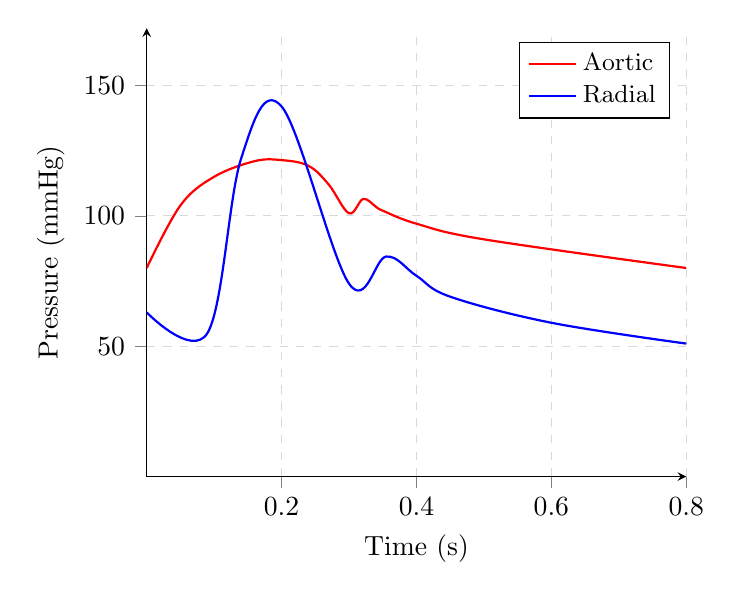
\begin{tikzpicture}
\begin{axis}[
        axis lines=middle,
        grid = major,
        grid style={dashed, gray!30},
	ymin = 0,
	ymax = 172,
	xmin = 0,
xmax =0.8,
        grid = major,
	 ylabel near ticks,
	xlabel near ticks,
        xlabel=Time (s),
        ylabel=Pressure (mmHg),
        tick align=outside,
        enlargelimits=false,
legend pos= north east,
legend style={font=\small, cells={align=left}},
legend cell align={left}
]

\draw[red,thick] plot[smooth,tension=0.6] 
coordinates { (axis cs: 0,80)
(axis cs: 0.05,104)
(axis cs: 0.1,115)
(axis cs: 0.16,121)
(axis cs: 0.2,121.4)
(axis cs: 0.24,119.2)
(axis cs: 0.27,112)
(axis cs: 0.30,101)
(axis cs: 0.321,106.5)
(axis cs: 0.34,103.5)
(axis cs: 0.35,102)
(axis cs: 0.4,97)
(axis cs: 0.5,91)
(axis cs: 0.8,80)};

\addlegendimage{red, thick};
\addlegendentry{Aortic};

\draw[blue,thick] plot[smooth,tension=0.6] 
coordinates { (axis cs: 0,63)
(axis cs: 0.09,55)
(axis cs: 0.14,122)
(axis cs: 0.2,142)
(axis cs: 0.3,74)
(axis cs: 0.355,84.4)
(axis cs: 0.4,77)
(axis cs: 0.45,69)
(axis cs: 0.6,59)
(axis cs: 0.8,51)};

\addlegendimage{blue, thick};
\addlegendentry{Radial};

\end{axis}
\end{tikzpicture}
\end{document}